\chapter{TINJAUAN PUSTAKA}

% Ubah konten-konten berikut sesuai dengan isi dari tinjauan pustaka

\section{Penelitian Terkait}

% Ubah paragraf berikut sesuai dengan penelitian lain yang terkait dengan tugas akhir
\subsection{Pengembangan Sistem Keamanan Berbagi Data PACS Berbasis Blockchain}
Penulis pada \parencite{DitoPrabowo2020} membuat sebuah sistem berbagi record data PACS pasien dalam penelitian ini
telah berhasil dalam mengintegrasikan record data pasien antar rumah sakit juga tambahan keamanan dengan pemberian akses untuk
berbagi, rumah sakit yang mendapat akses token dan secret key dapat membaca maupun menulis data pasien sesuai akses token yang
diberikan pasien. Bagi yang tidak mendapatkan akses tidak akan
bisa membaca maupun menulis data pasien, dengan ini keamanan
dan privasi pasien terjaga penuh. Kendali atas datanya tetap pasien yang menentukan. Kejadian data breach juga sulit dilakukan
pada sistem aplikasi yang bersifat desentralisasi dan menggunakan
platform \emph{blockchain} apalagi data juga dienkripsi.
Terkait dengan scalability, sistem mampu menangani berbagai size file yang beragam mulai dari 1Mb sampai dengan 64 Mb,
dan dari dilakukannya beberapa pengujian didapatkan hasil eksekusi waktu yang mendekati sama, dari ini bisa diketahui bahwa IPFS
stabil, juga bisa lebih cepat apabila file sudah pernah unggah sebelumnya (hash file sama).
Pada fitur aplikasi, semakin banyak data yang di buat block
akan semakin banyak waktu yang diperlukan untuk mining. Terbukti pada feature panambahan data pasien didapatkan rata-rata
waktu mining 0,51 detik, lebih lama dari feature yang lain.

\subsection{Securing music sharing platforms: A Blockchain-Based Approach}
Penulis pada paper \parencite{adjei2021securing} mengajukan sebuah platform berbagi musik yang berbasis pada \emph{blockchain} dan arsitektur IPFS.
Proposisi dari penulis adalah menghilangkan dan meminimalkan pembagian musik ilegal dari pembuat konten di seluruh
internet menggunakan teknologi \emph{blockchain} yang juga memfasilitasi pemeriksaan duplikat metadata di
Internet. Jaringan berbagi file ini dibangun berdasarkan \emph{blockchain} Ethereum yang menggunakan
cara mekanisme konsensus untuk mencapai tujuan yang dinyatakan dari \emph{smart contract} dengan cara yang cepat dan aman.
Simulasi penulis menyajikan berbagai langkah yang diperlukan untuk memvisualisasikan pengoperasian sistem yang diusulkan. Penulis memperkenalkan fitur pendaftaran dan kontrol akses yang ditambahkan ke protokol IPFS untuk memastikan bahwa
file musik memiliki hak cipta. \emph{Smart contract} memastikan bahwa persyaratan yang harus dipenuhi sebelumnya
mengakses file musik diberlakukan. Keadaan jaringan yang tahan-rusak ditunjukkan sedemikian rupa sehingga
setiap node yang berpartisipasi memastikan bahwa catatan yang disimpan pada file musik yang diunduh sesuai dengan yang diharapkan
pendapatan. Akuntabilitas pendapatan yang efektif dicapai dengan sistem yang diusulkan.

\subsection{A Study on Blockchain-based Music Distribution Framework: Focusing on Copyright Protection}

Penulis pada paper \parencite{kim2020study} mendesain dan mengimplementasikan sebuah \emph{blockchain} based music copyright distribution model.
Model yang diajukan mengatur aset-aset musik menjadi \emph{blocks} dan mendistribusikannya kepada node-node yang berpartisipasi dalam blockchain.
Jika kita ingin mendistribusikan musik, kita dapat mengakses platformnya dimanapun dan kapanpun dengan perangkat komputer maupun smartphone untuk mengakses dan
mendaftarkan musik. Di masa depan, apabila hukum dan sistemnya teratur kembali, beragam konten yang disimpan didalam \emph{blockchain} dapat mengelola copyrightnya.

\subsection{A Secure Data Sharing Platform Using \emph{Blockchain} and Interplanetary File System}
Pada paper ini \parencite{naz2019secure}, sebuah framework data sharing yang aman berbasis \emph{blockchain} dipersembahkan. Tujuan utama dari pengajuan skenario ini adalah untuk
memberikan keautentikan dan kualitas data kepada customer. Sebuah penyimpanan terdesentralisasi IPFS memberikan solusi untuk masalah pada sisi pemilik.
Data hash yang diterima oleh IPFS dienkripsi dengan SSS, jadi seorang customer yang belum mendepositkan harga konten digital, tidak dapat mengakses datanya.

\subsection{Blockchain-Based Data Sharing for Decentralized Tourism Destinations Recommendation System}
Penulis pada paper \parencite{hariadi2020} meneliti mengenai \emph{blockchain} untuk berbagi data rekomendasi tourisme.
Salah satu hal yang dibutuhkan wisatawan untuk merencanakan kegiatan wisatanya adalah sistem rekomendasi.
Sistem rekomendasi destinasi wisata pada penelitian ini memiliki tiga node utama yaitu user, server, dan sensor.
Setiap node membutuhkan kemampuan untuk \emph{sharing data} untuk menghasilkan rekomendasi yang diharapkan pengguna melalui perangkat seluler mereka.
Dalam makalah ini, diusulkan skema sistem \emph{data sharing} menggunakan jaringan desentralisasi berbasis blockchain yang setiap node dapat terhubung langsung satu sama lain, untuk mendukung pertukaran data di antara mereka. Arsitektur blok yang digunakan dalam jaringan blockchain memiliki tiga bagian utama, yaitu informasi blok, hash, dan data.

\section{Teori/Konsep Dasar}

\subsection{\emph{Blockchain}}

\emph{Blockchain} adalah database terdistribusi yang digunakan
untuk menangani record data yang terus bertambah, record data ini
disebut dengan block. Setiap block memiliki penanda waktu dan
kode unik yang terhubung dengan block sebelumnya, sehingga masing
masing block tersebut saling terhubung satu sama lainnya dan
tidak bisa untuk diubah.

\begin{figure} [ht] \centering
    % Nama dari file gambar yang diinputkan
    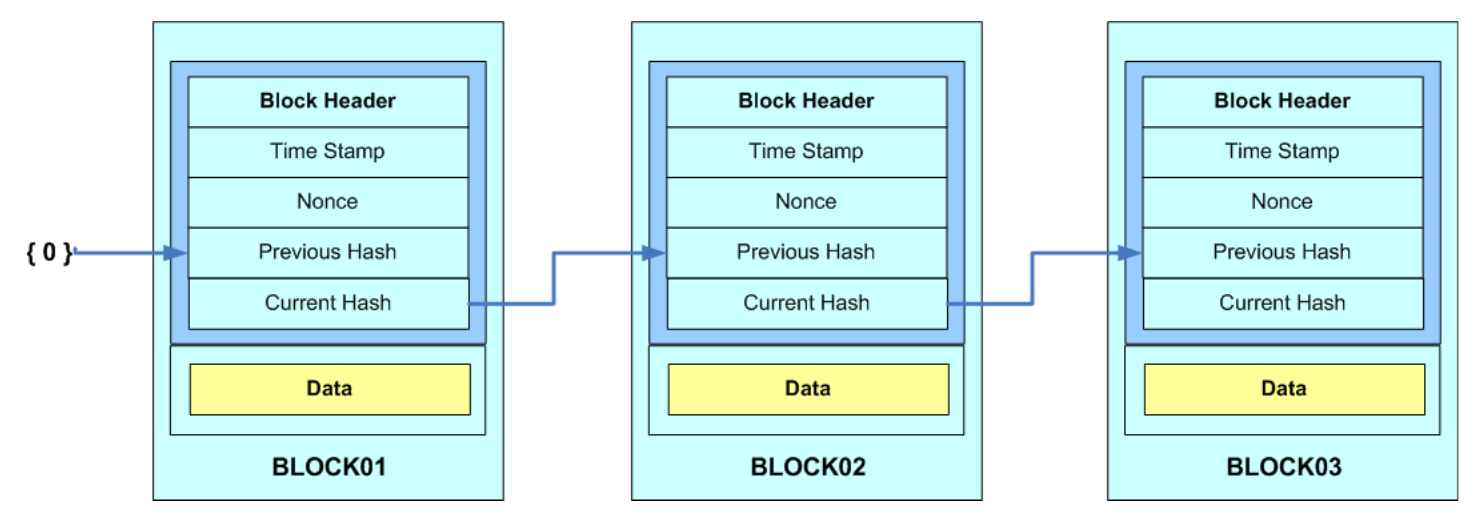
\includegraphics[scale=0.4]{gambar/blockchainanatomy.png}
    % Keterangan gambar yang diinputkan
    \caption{Blockchain Anatomy}
    % Label referensi dari gambar yang diinputkan
    \label{fig:blockchainanatomy}
\end{figure}

Bagan diatas adalah visualisasi dari anatomi \emph{blockchain}. Perlu diketahui
bahwa data dari \emph{blockchain} itu tidaklah di enkripsi, akan tetapi yang dienkripsi adalah
\emph{previous hash} dan \emph{current hash}-nya, dengan algoritma enkripsi yang berbeda-beda pada setiap implementasinya.
\emph{Blockchain} biasanya dikelola oleh jaringan
peer-to-peer yang secara kolektif mengikuti protokol untuk
memvalidasi block baru. Jika terdapat perintah penambahan block baru,
maka setiap node pada jaringan peer-to-peer tersebut akan terlebih
dahulu memvalidasi block dan kemudian seluruh node akan memperbarui record data miliknya [18]. \emph{Blockchain} memiliki 3 type \parencite{url:blockchaintype}
yaitu \emph{Public Blockchain} yang dikembangkan secara bersama-sama
oleh publik dan siapa saja dapat ikut serta untuk mengembangkan
blockchain, \emph{Private Blockchain} yang hanya bisa digunakan oleh
organisasi tertentu, \emph{consortium blockchain} yang dikembangkan oleh
suatu kelompok secara bersama untuk kepentingan tertentu,
sederhananya \emph{blockchain konsorsium} merupakan \emph{blockchain privat} yang
diberdayakan oleh lebih dari satu kelompok.

\subsection{\emph{Metaverse}}

Istilah metaverse pertama kali digunakan oleh Neal Stephenson di novelnya \emph{Snow Crash} untuk
mendeskripsikan dunia virtual dimana karakter protagonisnya, \emph{Hiro Protagonist}
, bersosialisasi, belanja, dan mengalahkan musuh-musuh dunia nyata melalui avatarnya. Ini bukanlah konsep yang baru
. Faktanya, film garapan Steven Spielberg pada tahun 2018 yang berjudul \emph{Ready Player One} juga mengambil konsep yang serupa dan
menggunakannya dengan sangat ciamik. Definisi teknis dari Metaverse itu sendiri adalah sebuah ruang virtual dimana orang-orang didalamnya bisa berinteraksi
dengan lingkungan yang dibuat oleh komputer dan pemain lain. Dalam penelitian ini implementasinya menggunakan
\emph{Unreal Engine 5}.

\subsection{\emph{NFT}}
NFT merupakan antarmuka standar untuk membuat \emph{Non Fungible Token}, atau NFT.
Use case untuk NFT adalah kepemilikan asset digital dan transaksinya hingga pengiriman ke
\emph{crypto wallet} pihak ketiga.

\subsection{\emph{Solidity}}
\emph{Solidity} adalah adalah bahasa tingkat tinggi berbasis objek untuk mengimplementasikan
\emph{smart contract}. Solidity ini dijalankan didalam \emph{Ethereum Virtual Machine (EVM)}.

\subsection{\emph{MetaSounds}}
MetaSounds merupakan plugin dari \emph{Unreal Engine 5} yang berfungsi sebagai sistem audio
berperforma tinggi yang menawarkan \emph{audio designers} dengan kendali penuh.

\subsection{\emph{Unreal Engine 5}}

Unreal Engine (UE) adalah Game Engine grafis komputer 3D yang dikembangkan oleh Epic Games, pertama kali dipamerkan dalam game penembak orang pertama tahun 1998 Unreal.
Awalnya dikembangkan untuk penembak orang pertama PC, sejak itu telah digunakan dalam berbagai genre permainan dan telah diadopsi oleh industri lain, terutama industri film dan televisi. Ditulis dalam C++,
Unreal Engine 5 dipublikasi pada tanggal 13 Mei 2020, mendukung semua sistem yang ada termasuk konsol generasi berikutnya PlayStation 5 dan Xbox Series X/S.\parencite{StattEpicAnnounce} Pengerjaan mesin dimulai sekitar dua
tahun sebelum diumumkan.\parencite{DeanTakahashi} UE5 dirilis dalam early access pada 26 Mei 2021,\parencite{EddieMakuch} dan secara resmi diluncurkan untuk pengembang pada 5 April 2022.\parencite{UE5Launch}

Salah satu fitur utamanya adalah Nanite, mesin yang memungkinkan bahan sumber fotografi dengan detail tinggi diimpor ke dalam game.\parencite{ValentineRebekah} Teknologi geometri tervirtualisasi Nanite memungkinkan Epic memanfaatkan akuisisi Quixel sebelumnya, perpustakaan fotogrametri terbesar di dunia pada 2019. Tujuan Unreal Engine 5 adalah untuk memudahkan pengembang
membuat dunia game yang mendetail tanpa harus menghabiskan banyak waktu untuk membuat aset detail baru.\parencite{DeanTakahashi} Nanite dapat mengimpor hampir semua representasi objek dan lingkungan tiga dimensi yang sudah ada sebelumnya, termasuk model ZBrush dan CAD, memungkinkan penggunaan aset berkualitas film.\parencite{AndrewTarantola} Nanite secara otomatis menangani tingkat detail (LODs)
dari objek yang diimpor ini sesuai dengan platform target dan jarak menggambar, tugas yang harus dilakukan oleh seorang seniman jika tidak.\parencite{KyleOrland} Lumen adalah komponen lain yang digambarkan sebagai "solusi iluminasi global yang sepenuhnya dinamis yang segera bereaksi terhadap pemandangan dan perubahan cahaya". Lumen menghilangkan kebutuhan
seniman dan pengembang untuk membuat peta cahaya untuk adegan tertentu, tetapi sebaliknya menghitung pantulan cahaya dan bayangan dengan cepat, sehingga memungkinkan perilaku sumber cahaya waktu nyata.\parencite{KyleOrland} Virtual Shadow Maps adalah komponen lain yang ditambahkan di Unreal Engine 5 yang digambarkan sebagai "metode pemetaan bayangan baru yang digunakan
untuk memberikan bayangan resolusi tinggi yang konsisten yang bekerja dengan aset berkualitas film dan dunia terbuka yang besar dan menyala secara dinamis"..\parencite{VirtualShadowMaps} Peta Bayangan Virtual berbeda dari implementasi peta bayangan pada umumnya dalam resolusi yang sangat tinggi, bayangan yang lebih detail, dan kurangnya bayangan yang muncul dan keluar yang
dapat ditemukan dalam teknik peta bayangan yang lebih umum karena kaskade bayangan.[121] Komponen tambahan termasuk Niagara untuk dinamika fluida dan partikel dan Chaos untuk mesin fisika.\parencite{DeanTakahashi}

\subsection{\emph{InterPlanetary File System}}

IPFS (InterPlanetary File System) adalah sebuah protocol dan
peer to peer jaringan untuk berbagi data dalam distributed file system. Cara kerjanya mirip seperti BitTorrent, yaitu bisa memperoleh
suatu data dari node node yang terhubung bukan dari server terpusat. Sistem pada IPFS bergantung pada distributed hash table
(DHT) untuk memperoleh lokasi data dan informasi konektifitas
antar node. Berdasarkan \parencite{Steichen2018}, berikut ini adalah gambaran bagaimana
IFPS bekerja. Ketika sebuah data di upload ke dalam IPFS, data tersebut
di pecah menjadi 5 bagian, masing-masing memiliki setidaknya
256 kilobytes data atau link ke chunk yang lain. Setiap chunk
diidentifikasi dengan \emph{cryptographic hash}, yang juga dinamakan \emph{content
    identifier}, yang telah dikomputasi dari kontennya sendiri. Link yang
di sebut juga mempunyai content identifiers, dan dengan demikian
akan membentuk \emph{Merkle directed acyclic graph (Merkle DAG)} yang
di deskripsikan dapat digunakan untuk reconstruct file apapun dari
chunk nya. Karena \emph{Merkle DAG}, keseluruhan data dapat
diidentifikasi hanya dengan menggunakan root hash nya. Karena IPFS
menggunakan content identifier untuk identifikasinya, bisa
mengirimkan content identifier ini ke dalam \emph{blockchain}, jadi tidak
menyimpan sebuah file dalam \emph{blockchain} tetapi menyimpannya dalam
IPFS dan melakukan query ke \emph{blockchain} untuk mendapatkan
hashnya yang kemudian direkonstruksi menjadi sebuah data. Dan
pastinya tidak ada duplikasi serta setiap data tentunya akan memiliki
hash yang berbeda beda ketika data di submit dalam IPFS.
